\section{Durchführung}
\label{sec:Durchführung}

%Zu jedem Bild, jeder Tabelle, jeder Abbildung im allgemeinen einen Satz schreiben





\begin{figure}[H]
    \centering
    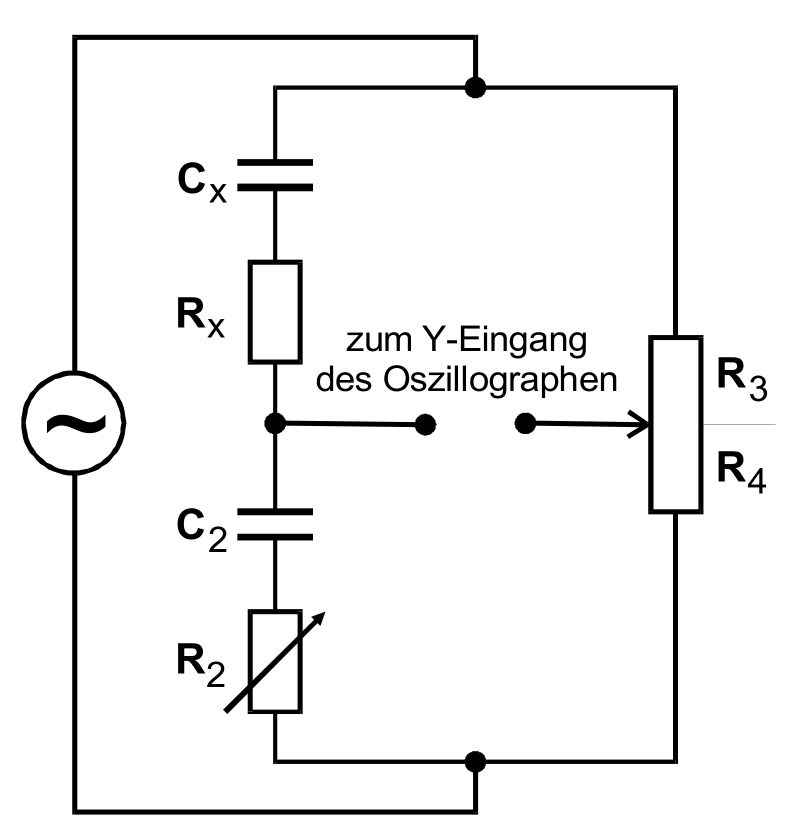
\includegraphics[width=0.75\textwidth]{dateien/aufgabeb).png}
    \caption{Schaltplan einer Kapazitätsmessbrücke \cite{anleitung}.}
    \label{fig:schaltungb}
\end{figure}

\begin{figure}[H]
    \centering
    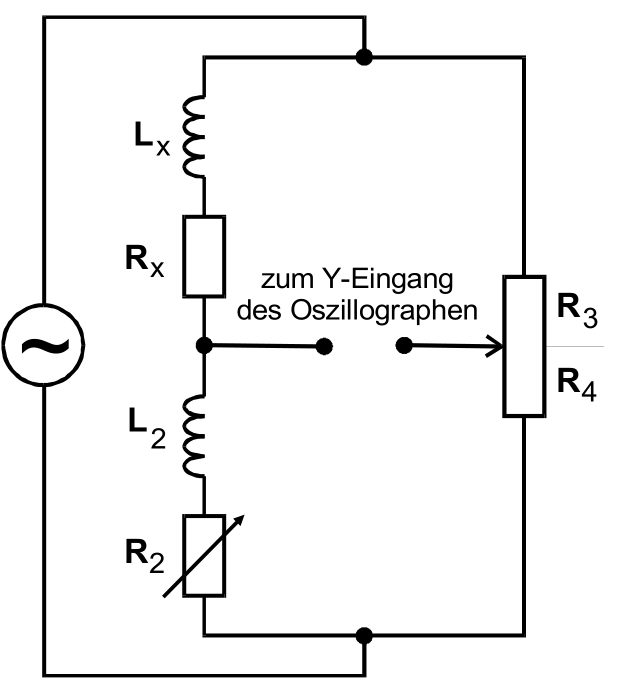
\includegraphics[width=0.75\textwidth]{dateien/aufgabec).png}
    \caption{Schaltplan einer Messbrücke für verlustbehaftete Induktivitäten \cite{anleitung}.}
    \label{fig:schaltungc}
\end{figure}

\begin{figure}[H]
    \centering
    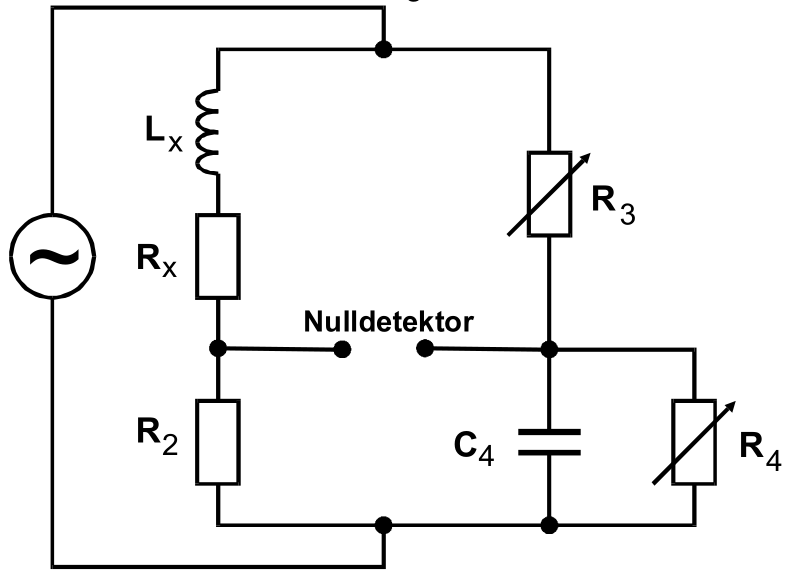
\includegraphics[width=0.75\textwidth]{dateien/aufgabed).png}
    \caption{Schaltplan einer Maxwell-Brücke \cite{anleitung}.}
    \label{fig:schaltungd}
\end{figure}

\begin{figure}[H]
    \centering
    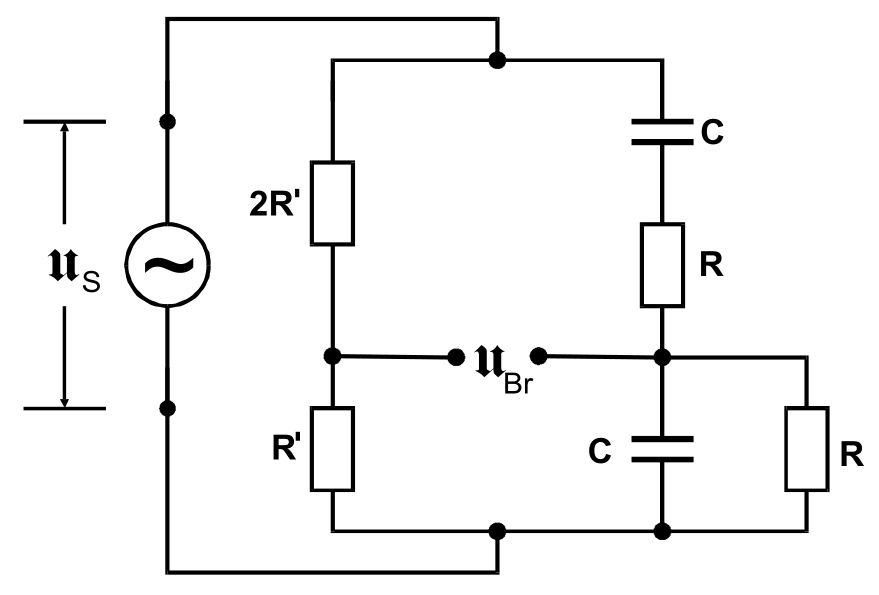
\includegraphics[width=0.75\textwidth]{dateien/aufgabee).png}
    \caption{Schaltplan einer Wien-Robinson-Brücke \cite{anleitung}.}
    \label{fig:schaltunge}
\end{figure}